\workshopexclude{\section{Quantitative Analysis}}
\workshoponly{\section{Additional Results - Quantitative Analysis}}
In this section, we conduct quantitative analyses to better understand the three main components of our method: proposal distribution, score functions, and iterative search. Moreover, we conduct a cost analysis in the Appendix \ref{sec:cost_analysis} to understand the most cost-efficient way to find the best prompt. We observe the larger and more powerful language models are more cost-effective for generating the best prompt despite a higher per-token cost.

\subsection{LLMs for Proposal Distribution}

\paragraph{How does the proposal quality change as we increase the model size?} To understand how the model size affects the quality of the initial proposal distribution, we examine eight different models\footnote{We use ada, babbage, curie, davinci, text-ada-001, text-babbage-001, text-curie-001, text-davanci-002} available via the OpenAI API. To assess the quality of the proposal distribution, we generate 250 instructions per model and compute the execution accuracy on 50 test data points. We visualize the survival function (percentage of instructions with test accuracy greater than a certain threshold) and the histogram of test accuracy for a simple task (i.e., Pluralization) in Figure \ref{fig:main-posterior} (a) and include a similar plot for a more challenging task (Start With) in the Appendix (Figure \ref{fig:app-posterior-model-size-hard}). As shown in both figures (and unsurprisingly), larger models tend to produce better proposal distributions than smaller ones, as do the models that were fine-tuned to follow human instructions. On the simple task, all instructions generated by the best model, InstructGPT (175B), have reasonable test accuracy. In contrast, half of the instructions are off-topic and perform poorly on the more challenging task. 

\begin{figure}
  \centering
  \vspace{-0.1in}
 \begin{subfigure}[b]{0.49\textwidth}
  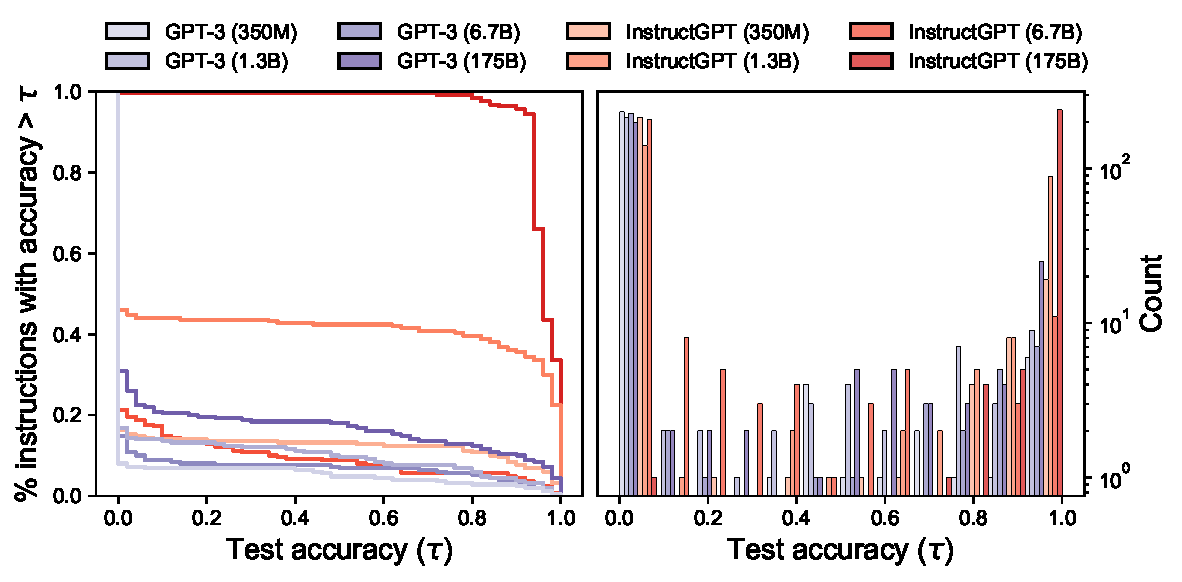
\includegraphics[width=1.0\linewidth]{figures/main/posterior_model_size_plural.pdf}
  \end{subfigure}
  \begin{subfigure}[b]{0.49\textwidth}
  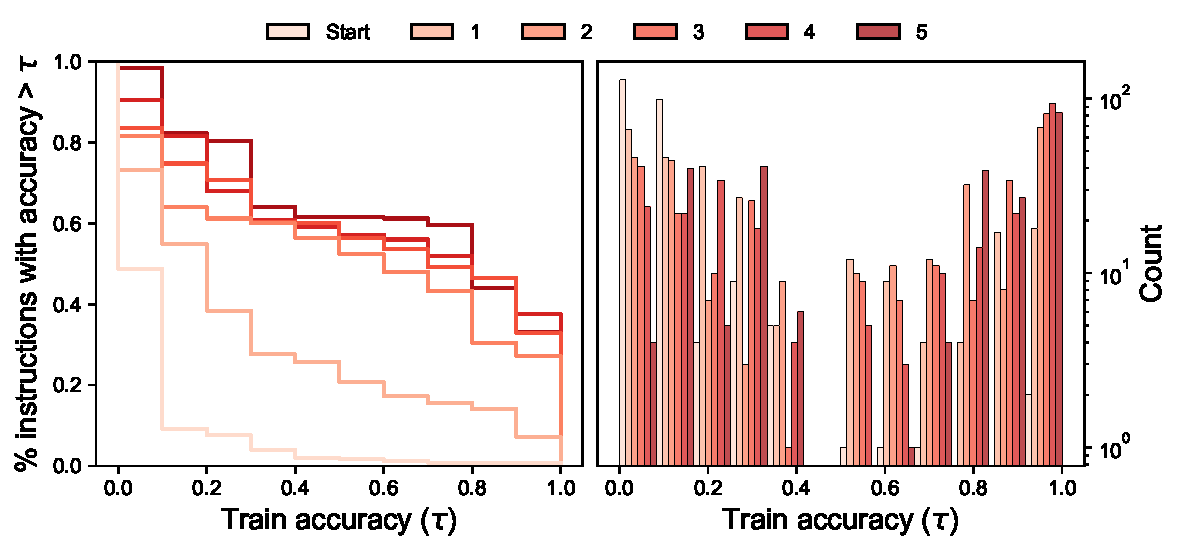
\includegraphics[width=1.0\linewidth]{figures/main/posterior_mcmc_passive.pdf}
  \end{subfigure}
  \caption{(Left) Quality of the proposal distribution of models with different size as assessed by test execution accuracy. (Right) Iterative Monte Carlo search improves the quality of the instruction candidates at each round.}\label{fig:main-posterior}
\end{figure}

% \paragraph{Can we use other LLMs for instruction proposal?} We investigate other LLMs for instruction generation, including those with forward generation ability (OPT-175B \citep{zhang2022opt}, OpenAI Codex \citep{chen2021evaluating}) and one with reverse generation ability (INT4 quantized GLM-130B \citep{glm130b}).
% We evaluate their performance on six tasks selected from instruction induction on both zero-shot and few-shot settings \footnote{These six tasks are chosen such that two of them are worse than humans, and the other four are human-level. They cover six categories (spelling, morphosyntax, lexical semantics, semantics, multi-lingual, and GLUE).\label{sixtasks}}. Figures \ref{fig:app-zero-shot-diff-encoder} and \ref{fig:app-few-shot-diff-encoder} show that InstructGPT achieves the best performance except for passivization, where it underperforms compared to the two other forward-generation models. Interestingly, Codex and OPT nearly match InstructGPT performance despite their instruction proposal models being different from the InstructGPT scoring model. However, we observe some of the instructions generated by OPT contain in-context examples (Table \ref{tab:opt_instructions}), making them closer to few-shot rather than a zero-shot. In contrast, GLM achieves the poorest zero-shot performance as its infilling capabilities are trained to generate very short text, as shown in Table \ref{tab:glm_instructions}. 

% \paragraph{How important is the meta prompt?}
% As shown in Table \ref{tab:human-level-perf-summary}, the insert variant of InstructGPT underperforms compared to the forward variant, despite it being more intuitive to perform reverse generation from demonstrations. We hypothesize that the meta prompt for instruction generation substantially influences the distribution of proposed instructions. To this end, we experiment with our TruthfulQA template instead of the reverse generation template (Figures \ref{fig:app-zero-shot-meta_prompt}, \ref{fig:app-zero-shot-meta_prompt-best}, \ref{fig:app-few-shot-meta_prompt}, \ref{fig:app-few-shot-meta_prompt-best}). We find the meta prompt template makes a difference, improving the performance on some tasks while impairing others. Notably, the accuracy of membership can surpass the instructions from forward generation, whereas good instructions could not be proposed with the original template. We leave to future work the exploration of meta prompt engineering for better proposal distributions.

\subsection{LLMs for selection}
\paragraph{Does proposal quality matter under selection?} If we sample more instructions from the LLMs, then it becomes more likely for us to find better instructions. To verify this hypothesis, we increase the sample size from 4 to 128 and evaluate the test accuracy change. Figure \ref{fig:mcmc_comparison} (Left) shows a monotonically increasing trend with a diminishing return, as human-level performance is achieved with 64 instruction samples. Thus, we choose 50 as our default sample size. Under this configuration, we investigate how the proposal distribution affects the test accuracy of the best instruction selected by our algorithm. Figure \ref{fig:highlight}(b) shows that though the small models may be less likely to generate good instructions, they nonetheless generate some good ones if we sample enough candidates. Therefore, we still find promising instructions with a small model by running our selection algorithm, explaining why our method outperforms the greedy approach \cite{honovich2022instruction} across all eight models.

\paragraph{Which scoring function is better?} We compute the correlation between the test accuracy and two metrics on 24 instruction induction tasks to study how good our proposed metrics are. We generate 250 instructions per task using InstructGPT (175B) in “forward” mode and compute the metric score and test accuracy on 10 test data points. We visualize the Spearman correlation between the test accuracy and two metrics. Figure \ref{fig:mcmc_comparison} (Middle) shows that the execution accuracy aligns better with the test performance across the tasks. Thus, we choose it as our default metric unless otherwise stated.

% \paragraph{How transferable are the generated instructions?} We investigate whether \algname can be used to steer the model not involved in the instruction generation and selection process. As shown in Figure \ref{fig:app-zero-shot-diff-decoder}, there is a significant performance drop when we use the instructions from InstructGPT to steer the GPT-3 model, and vice versa. This performance drop can be mitigated by a human written instruction. It suggests that the alignment between the scoring model and execution model is crucial, and the instructions generated by InstructGPT work best for the InstructGPT itself but do not transfer well to a different model like GPT-3. In contrast, GPT-3-generated instructions can steer GPT-3 exceptionally well, outperforming the InstructGPT instructions and human instructions by a large margin. Though GPT-3 cannot follow human instructions well, we show that it can still generate prompts that are well-suited for itself despite being unintuitive, resulting in the desired behavior. We provide the generated prompts in Table \ref{tab:davinci-self}.

\begin{figure}
  \vspace{-0.15in}
  \centering
  \begin{subfigure}[b]{0.31\textwidth}
  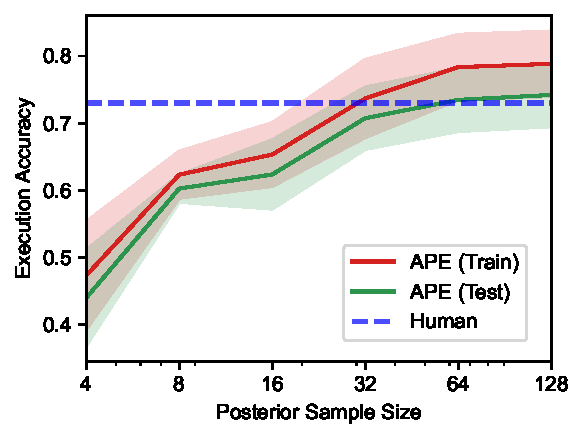
\includegraphics[width=1.0\linewidth]{figures/main/sample_size_task_mean.pdf}
  \end{subfigure}\hfill
 \begin{subfigure}[b]{0.31\textwidth}
  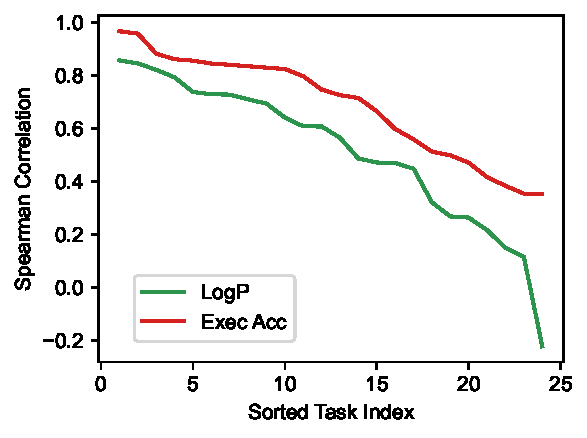
\includegraphics[width=1.0\linewidth]{figures/main/corr_metric_spearman.pdf}
  \end{subfigure}\hfill
   \begin{subfigure}[b]{0.31\textwidth}
  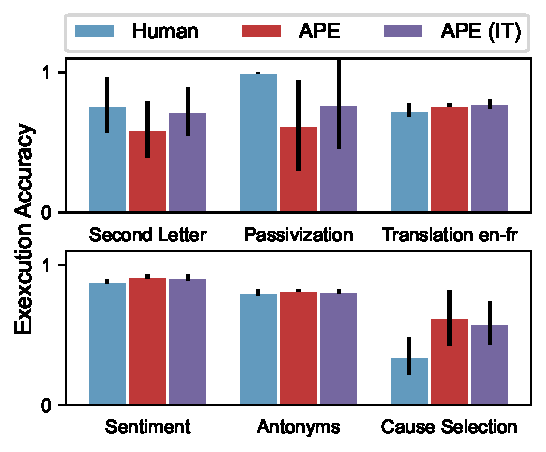
\includegraphics[width=1.0\linewidth]{figures/main/mcmc_comparison.pdf}
  \end{subfigure}
  \caption{(Left) Test execution of the best instruction as we increase the number of instruction candidates. We report the mean and standard deviation across 6 different tasks. (Middle) Spearman Correlation between the test accuracy and two metrics on 24 tasks. (Right) Test execution accuracy of the best instruction selected using \algname and iterative \algname (\algname (IT)).}\label{fig:mcmc_comparison}
  \vspace{-0.1in}
\end{figure}
\subsection{Iterative Monte Carlo Search}\label{ab:tmcs}
\paragraph{Does Iterative Search improve the instruction quality?} We visualize the survival function and histogram of test accuracy on the ``Passivization'' task in Figure \ref{fig:main-posterior} (Right) and include five more tasks in the Appendix. The survival plot shows that the curves increase as the round goes up, which suggests that iterative search does result in a higher-quality proposal set. However, we observe diminishing returns to further selection rounds as the quality seems to stabilize after three rounds.

\paragraph{Do we need Iterative Search?}
% Similar to what we have seen in the role the big model plays in performance, it is likely that a high-quality set of instruction candidates may not give us much performance gain. 
We compare \algname~and iterative \algname~on six tasks\footref{sixtasks}. As shown in Figure \ref{fig:mcmc_comparison}, the iterative search marginally improves performance on tasks where APE underperforms humans but achieves similar performance on the other tasks. This is consistent with our hypothesis that iterative search would be most useful on tasks where generating a good initial $\proposal$ is challenging.